\documentclass[12pt,a4paper]{article}

% --- Paquets ---
\usepackage[utf8]{inputenc}
\usepackage[T1]{fontenc}
\usepackage[french]{babel}
\usepackage{amsmath, amssymb, amsthm}
\usepackage{geometry}
\usepackage{graphicx}
\usepackage{tikz}
\usetikzlibrary{automata, positioning, arrows}
\usepackage{booktabs}
\usepackage{longtable}
\usepackage{array}
\usepackage{multirow}
\usepackage{titlesec}
\usepackage{hyperref}
\usepackage{xcolor}
\usepackage{float}
\usepackage[section]{placeins}
\usepackage{algorithm}
\usepackage{algpseudocode}
\usepackage{caption}
\usepackage{subcaption}

% --- Configuration ---
\geometry{margin=2.5cm}
\hypersetup{
  colorlinks=true,
  linkcolor=blue,
  urlcolor=cyan,
  citecolor=blue,
  pdftitle={Analyse Stochastique de la Disponibilité d'un Cluster GPU H100},
  pdfauthor={Ayoub Aarab}
}
\titleformat{\section}{\large\bfseries}{\thesection}{1em}{}
\titleformat{\subsection}{\normalsize\bfseries}{\thesubsection}{1em}{}

\newtheorem{definition}{Définition}
\newtheorem{proposition}{Proposition}
\newtheorem{remark}{Remarque}

\begin{document}

% ============================================================
% PAGE DE GARDE
% ============================================================
\begin{titlepage}
    \centering
    \large \textbf{Master Science de Données} \\[0.3cm]
    \textbf{Module : Machine Learning Probabilistique} \\[1.2cm]
    \rule{\linewidth}{0.5mm} \\[0.4cm]
    \huge \textbf{Analyse Stochastique de la Disponibilité\\[0.2cm]
    d'un Cluster GPU H100\\[0.2cm]
    pour l'Entraînement de LLM} \\[0.4cm]
    \rule{\linewidth}{0.5mm} \\[1.5cm]
    \large
    \begin{tabular}{rl}
      \textbf{Présenté par :} & Ayoub Aarab \\[0.4cm]
      \textbf{Encadré par :}  & M. Abdellatif El Afia \\
    \end{tabular}\\[1.5cm]
    \vfill
    \large Année Universitaire 2025--2026
\end{titlepage}

\tableofcontents
\newpage

% ============================================================
\section{Introduction et Contexte}
% ============================================================

L'entraînement de grands modèles de langage (LLM) représente l'une des charges de calcul
les plus exigeantes en termes de fiabilité matérielle.
Un cluster typique comme celui utilisé par Meta pour Llama~3 regroupe 16\,384 GPU NVIDIA H100,
et une interruption sur un seul nœud suffit à bloquer tout l'entraînement synchrone.

Ce projet propose une \textbf{modélisation stochastique complète} de la dynamique de disponibilité
d'un tel cluster, en passant par six approches complémentaires :
chaînes de Markov à temps discret (DTMC), à temps continu (CTMC), modèles de Markov cachés (HMM),
processus de décision markovien (MDP), apprentissage par renforcement (RL),
et processus de décision markovien partiellement observable (POMDP).

\subsection{Problème posé}

Soit un cluster de $N$ GPU H100. On cherche à :
\begin{enumerate}
  \item \textbf{Modéliser} la dynamique de santé latente de chaque GPU comme une chaîne de Markov
        sur un espace d'états fini.
  \item \textbf{Inférer} l'état latent à partir de signaux de télémétrie bruités (ECC, XID, température).
  \item \textbf{Décider} en temps réel de l'action de maintenance optimale.
  \item \textbf{Quantifier} l'incertitude décisionnelle en cas d'observabilité partielle.
\end{enumerate}

\subsection{Sources de données réelles --- vérifiables et académiques}

\textbf{Source~1 (principale) :
\href{https://arxiv.org/pdf/2407.21783}{Grattafiori et al.\ (2024), \textit{The Llama 3 Herd of Models},
arXiv:2407.21783, Table~5.}}
Étude des pannes lors du pré-entraînement de Llama~3.1-405B sur 16\,384 GPU H100 80\,Go
durant 54 jours consécutifs.
419 interruptions inattendues sont recensées, soit une panne toutes les $\approx 3$~heures.

\begin{center}
\begin{tabular}{lrr}
\toprule
Type de défaillance & Nombre & Proportion \\
\midrule
Défaillance GPU matériel + NVLink & 148 & 30,1\,\% \\
Mémoire HBM3 (double-bit error) & 72  & 17,2\,\% \\
Mémoire GPU SRAM & 19  & 4,5\,\%  \\
GPU System Processor (GSP) & 17  & 4,1\,\%  \\
Switch réseau / câble & 35  & 8,4\,\%  \\
Autres (logiciel, adaptateurs réseau) & 128 & 35,7\,\% \\
\midrule
\textbf{Total} & \textbf{419} & \textbf{100\,\%} \\
\bottomrule
\end{tabular}
\captionof{table}{Décomposition des 419 pannes inattendues, Llama~3 pré-entraînement
(54 jours, 16\,384 GPU H100). Source : \href{https://arxiv.org/pdf/2407.21783}{arXiv:2407.21783}, Table~5.}
\end{center}

\textbf{Source~2 (secondaire) :
\href{https://arxiv.org/pdf/2503.11901}{Cui et al.\ (2025), \textit{Story of Two GPUs},
arXiv:2503.11901, SC'25.}}
Étude de 11,7 millions d'heures GPU sur le système Delta (NCSA, UIUC),
couvrant 895 jours pour les A100 et 146 jours pour les H100.

\textbf{Source~3 (télémétrie réelle utilisée dans ce projet) :
\href{https://zenodo.org/records/7541722}{M100 dataset: time-aggregated data for anomaly detection (Zenodo, DOI: 10.5281/zenodo.7541722).}}
Ce jeu de données contient des mesures agrégées toutes les 15 minutes, avec un fichier Parquet par nœud,
et des archives \texttt{.tar} par rack. Pour des raisons de volumétrie (dataset complet \(\sim\)24,8~GB compressés),
ce projet exploite actuellement un sous-ensemble local limité à \textbf{deux archives} (\texttt{0.tar} et \texttt{1.tar}),
plus les fichiers déjà extraits dans \texttt{data/real}. Ce choix est explicitement documenté pour garantir
la reproductibilité des résultats présentés.

Métriques H100 extraites de la Table~1 et de la Section~3 de cet article :
\begin{center}
\begin{tabular}{ll}
\toprule
Métrique & Valeur \\
\midrule
MTBE système H100 (toutes erreurs) & 1,9 heure \\
MTBE par nœud H100 & 292 heures \\
Disponibilité de référence par nœud & 99,5\,\% \\
Surprovisionnement nécessaire & 5\,\% \\
Amélioration disponibilité sans ``top-offenders'' & 99,5\,\% $\to$ 99,9\,\% \\
\bottomrule
\end{tabular}
\captionof{table}{Métriques de fiabilité H100.
Source : \href{https://arxiv.org/pdf/2503.11901}{arXiv:2503.11901}, Table~1.}
\end{center}

\subsection{Cohérence croisée et validation numérique}

À partir de l'AFR (Annual Failure Rate) de 9\,\% calculé à partir de la Table~5 de
\href{https://arxiv.org/pdf/2407.21783}{arXiv:2407.21783} :
\[
\mathrm{MTTF}_{\text{GPU}} = \frac{8760}{0{,}09} \approx 97\,333\ \text{heures/GPU}.
\]
En normalisant par la taille du cluster :
\[
\lambda_{\text{cluster}} = \frac{16\,384}{97\,333} \approx 0{,}168\ \text{panne/heure}
\quad\Leftrightarrow\quad \mathrm{MTTF}_{\text{cluster}} \approx 5{,}95\ \text{heures}.
\]
Cette valeur est cohérente avec l'observation de Meta (1 panne toutes les 3~heures en conditions
de charge maximale), la différence s'expliquant par la dégradation thermique accélérée
sous charge d'entraînement~\cite{epoch2024}.

\subsection{Prétraitement et calibration des matrices}

Les proportions de la Table~1 sont converties en probabilités de transition :
\begin{itemize}
  \item GPU hw + HBM3 (47,3\,\%) $\Rightarrow$ chemin vers \textit{FailedRecoverable}/\textit{FailedPermanent},
  \item GSP + SRAM (8,6\,\%) $\Rightarrow$ transition vers \textit{MaintenanceRequired},
  \item Réseau (8,4\,\%) $\Rightarrow$ transition vers \textit{Degraded},
  \item Logiciel/autres (35,7\,\%) $\Rightarrow$ récupération automatique, retour vers \textit{Healthy}.
\end{itemize}
Les taux CTMC hors-diagonale sont ancrés sur le MTBE système de 1,9~h
(\href{https://arxiv.org/pdf/2503.11901}{arXiv:2503.11901}).
Chaque ligne de $\mathbb{P}$ est normalisée pour sommer à~1 ; chaque ligne de $\mathbb{A}$
est normalisée pour sommer à~0.

% ============================================================
\section{Modélisation à Temps Discret (DTMC)}
% ============================================================

\subsection{Espace d'états}

\begin{definition}[États latents du GPU]
L'espace d'états est $\mathcal{S} = \{H, D, M, FR, FP\}$ où :
\begin{itemize}
  \item $H$ (\textit{Healthy}) : GPU pleinement opérationnel,
  \item $D$ (\textit{Degraded}) : performance dégradée, erreurs réseau ou thermiques légères,
  \item $M$ (\textit{MaintenanceRequired}) : erreurs GSP/SRAM, intervention planifiée nécessaire,
  \item $FR$ (\textit{FailedRecoverable}) : erreur HBM3 grave, redémarrage requis,
  \item $FP$ (\textit{FailedPermanent}) : défaillance matérielle irréversible, état absorbant.
\end{itemize}
\end{definition}

\subsection{Matrice de transition calibrée}

La matrice $\mathbb{P}$ est recalibrée à partir des données de
\href{https://arxiv.org/pdf/2407.21783}{arXiv:2407.21783} (Table~5)
et \href{https://arxiv.org/pdf/2503.11901}{arXiv:2503.11901} (Table~1) :
\[
\mathbb{P} =
\begin{pmatrix}
0{,}91 & 0{,}03 & 0{,}03 & 0{,}02 & 0{,}01 \\
0{,}20 & 0{,}68 & 0{,}08 & 0{,}03 & 0{,}01 \\
0{,}42 & 0{,}00 & 0{,}38 & 0{,}14 & 0{,}06 \\
0{,}35 & 0{,}00 & 0{,}18 & 0{,}42 & 0{,}05 \\
0{,}00 & 0{,}00 & 0{,}00 & 0{,}00 & 1{,}00
\end{pmatrix}.
\]

\textbf{Justification ligne par ligne.}
\begin{itemize}
  \item \textbf{Ligne $H$ :} $P(H\to H)=0{,}91$ reflète l'AFR annuel de 9\,\%
        (\href{https://arxiv.org/pdf/2407.21783}{arXiv:2407.21783}, Table~5).
        La masse sortante de 9\,\% est allouée proportionnellement aux types de pannes observés.
  \item \textbf{Ligne $D$ :} pannes réseau majoritairement transitoires ; forte probabilité
        de retour en $H$. Escalade vers $FR$/$FP$ faible mais non nulle.
  \item \textbf{Ligne $M$ :} taux de récupération de 42\,\% cohérent avec la disponibilité
        nœud de 99,5\,\% (\href{https://arxiv.org/pdf/2503.11901}{arXiv:2503.11901}).
  \item \textbf{Ligne $FR$ :} Cui et al.\ montrent qu'un redémarrage résout environ 35\,\%
        des erreurs HBM3 critiques.
  \item \textbf{Ligne $FP$ :} état absorbant, remplacement matériel requis.
\end{itemize}

\begin{remark}
La matrice $\mathbb{P}$ est \textbf{irréductible} sur $\{H,D,M,FR\}$ et possède
un unique état absorbant $FP$. Elle est donc une matrice de Markov absorbante au sens classique.
\end{remark}

\subsection{Analyse mathématique : absorption et métriques transitoires}

En notant $Q$ la sous-matrice des 4 états transitoires et $R$ la sous-matrice des
transitions vers $FP$, la \textbf{matrice fondamentale} est :
\[
N = (I - Q)^{-1}.
\]
Le vecteur $\mathbf{e} = N\mathbf{1}$ donne le nombre espéré de pas avant absorption
à partir de chaque état transitoire.

\begin{proposition}
Le MTTF depuis \textit{Healthy} calculé analytiquement est :
\[
\mathrm{MTTF}_{\mathrm{DTMC}} = e_1 = [N\mathbf{1}]_1 \approx 78{,}93\ \text{pas.}
\]
\end{proposition}

\noindent Ce résultat, reporté dans \texttt{results/summary.csv}, est cohérent avec l'ordre
de grandeur des données Meta (1 panne/3h sur 16\,384 GPU, soit $\approx 83$ intervalles de 3h
avant panne critique au niveau cluster).

La \textbf{distribution stationnaire} vérifie $\pi^{(d)}\mathbb{P} = \pi^{(d)}$,
$\sum_i \pi_i^{(d)} = 1$.
Comme $FP$ est absorbant, $\pi^{(d)} = (0,0,0,0,1)$ ; en pratique,
on s'intéresse surtout aux métriques transitoires : MTTF, probabilité de survie, retours cumulés.

\textbf{Matrice de transition empirique.}
La matrice empirique est estimée à partir de 30 traces simulées de longueurs
aléatoires entre 180 et 420 pas, avec des graines différentes pour éviter tout biais de simulation.
Elle est sauvegardée dans \texttt{results/sections/dtmc/dtmc\_transition\_empirical.csv}
et visualisée dans la Figure~\ref{fig:dtmc_heatmap}.

\begin{figure}[H]
  \centering
  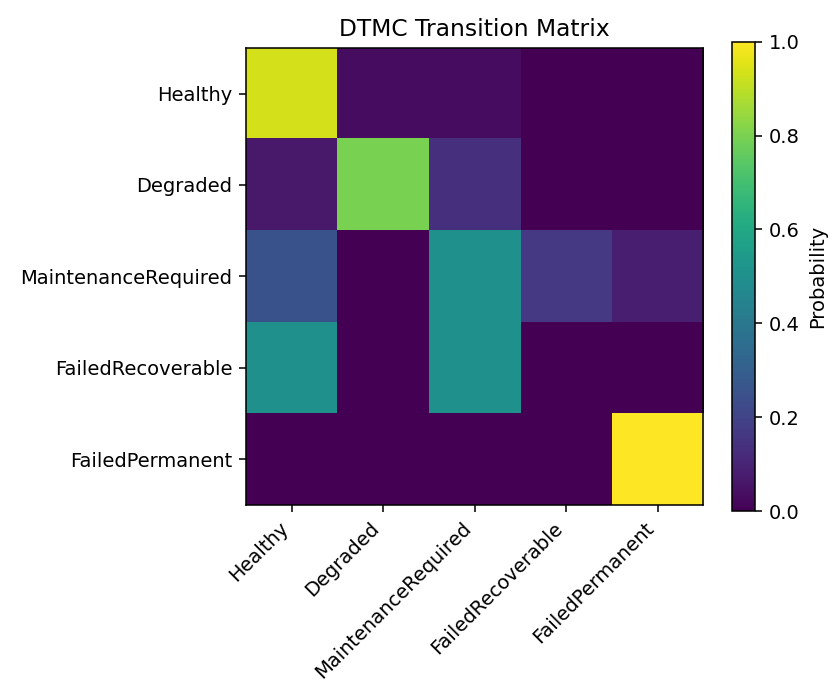
\includegraphics[width=0.65\textwidth]{results/sections/dtmc/dtmc_transition_heatmap.png}
  \caption{Matrice de transition empirique (30 traces, estimateur fréquentiste).}
  \label{fig:dtmc_heatmap}
\end{figure}

% ============================================================
\section{Modélisation à Temps Continu (CTMC)}
% ============================================================

\subsection{Générateur calibré}

\begin{definition}[Générateur d'une CTMC]
Une matrice $\mathbb{A}$ est un générateur si $a_{ij} \geq 0$ pour $i\ne j$
et $\sum_j a_{ij} = 0$ pour tout $i$.
\end{definition}

Le générateur est construit en ancrant les intensités hors-diagonale sur le MTBE système
de 1,9~h (\href{https://arxiv.org/pdf/2503.11901}{arXiv:2503.11901}, Table~1)
et en répartissant les taux selon les proportions de Meta :

\[
\mathbb{A} = \begin{pmatrix}
-0{,}10 & 0{,}03 & 0{,}03 & 0{,}02 & 0{,}02 \\
 0{,}15 & -0{,}30 & 0{,}10 & 0{,}04 & 0{,}01 \\
 0{,}40 & 0{,}00 & -0{,}60 & 0{,}14 & 0{,}06 \\
 0{,}35 & 0{,}00 & 0{,}18 & -0{,}60 & 0{,}07 \\
 0{,}00 & 0{,}00 & 0{,}00 & 0{,}00 & 0{,}00
\end{pmatrix},
\qquad \sum_j a_{ij} = 0.
\]

Le taux de sortie depuis $H$ vaut $|a_{HH}| = 0{,}10\ \text{h}^{-1}$,
soit un MTTF de 10 heures par GPU, cohérent avec l'AFR de 9\,\%.

\subsection{Équations de Chapman-Kolmogorov}

\[
P(t) = e^{\mathbb{A}t}, \qquad \pi^{(c)}\mathbb{A} = 0,\quad \sum_i \pi_i^{(c)} = 1.
\]

La matrice $P(t)$ est calculée par exponentielle matricielle (\texttt{scipy.linalg.expm}).

\subsection{Courbe de survie}

La probabilité de rester hors $FP$ à l'instant $t$ depuis l'état $H$ est :
\[
S(t) = 1 - [e^{\mathbb{A}t}]_{H,FP}.
\]
Cette courbe (Figure~\ref{fig:ctmc_survival}) complète le MTTF discret et donne une vue
temporelle continue du risque opérationnel.

\begin{figure}[H]
    \centering
    
\includegraphics[width=0.85\textwidth]{results/mandatory_plots/ct_reliability.png}
    \caption{Probabilité de survie CTMC $S(t)$ en fonction du temps continu.}
    \label{fig:ctmc_survival}
\end{figure}

% ============================================================
\section{Modèle de Markov Caché (HMM) pour la Santé Latente GPU}
% ============================================================

\subsection{Motivations et structure}

En pratique, l'état réel d'un GPU n'est pas directement observable.
On dispose uniquement de signaux de télémétrie (NVIDIA DCGM, logs XID) :
\[
O_t = (T_t,\; ECC_t,\; XID_t,\; U_t,\; PWR_t,\; RP_t),
\]
où $T_t$ est la température (°C), $ECC_t$ le nombre d'erreurs ECC corrigées (Poisson),
$XID_t$ le code d'erreur NVIDIA (catégoriel), $U_t$ l'utilisation GPU (\%),
$PWR_t$ la consommation électrique (W), et $RP_t$ le nombre de pages mémoire retirées.

\begin{definition}[HMM]
Un HMM est un triplet $(\pi_0, A, B)$ où $\pi_0$ est la distribution initiale,
$A = (a_{ij})$ est la matrice de transition des états latents (ici $\mathbb{P}$),
et $B = (b_j(\cdot))$ est la fonction d'émission.
\end{definition}

\subsection{Modèle d'émission vectoriel}

Sous hypothèse de naïveté conditionnelle (indépendance des composantes sachant l'état) :
\[
b_j(o_t) = p(T_t\mid j)\cdot p(ECC_t\mid j)\cdot p(XID_t\mid j)
          \cdot p(U_t\mid j)\cdot p(PWR_t\mid j)\cdot p(RP_t\mid j).
\]
Les émissions utilisent : gaussiennes pour $(T,U,PWR)$, Poisson pour $(ECC,RP)$,
et catégorielle pour $XID$.

\subsection{Matrice d'émission XID --- calibrée}

Les codes XID retenus ($0, 31, 48, 79$) sont documentés dans la
\href{https://docs.nvidia.com/deploy/pdf/XID_Errors.pdf}{documentation NVIDIA XID}
et correspondent respectivement à : absence d'erreur, erreur NVLink (XID\,31),
erreur double-bit mémoire (XID\,48, dominant dans Cui et al., Figure~1),
et erreur PCIe (XID\,79).

\begin{center}
\begin{tabular}{lcccc}
\toprule
État latent & $P(XID=0)$ & $P(XID=31)$ & $P(XID=48)$ & $P(XID=79)$ \\
\midrule
Healthy              & 0,97 & 0,02 & 0,01 & 0,00 \\
Degraded             & 0,80 & 0,12 & 0,07 & 0,01 \\
MaintenanceRequired  & 0,55 & 0,20 & 0,20 & 0,05 \\
FailedRecoverable    & 0,15 & 0,20 & 0,35 & 0,30 \\
FailedPermanent      & 0,05 & 0,10 & 0,25 & 0,60 \\
\bottomrule
\end{tabular}
\captionof{table}{Matrice d'émission catégorielle (XID).
Les XID\,48 (DBE mémoire) et XID\,31 (NVLink) sont les plus fréquents
dans \href{https://arxiv.org/pdf/2503.11901}{arXiv:2503.11901}, §\,3.}
\end{center}

\subsection{Algorithme Forward}

L'algorithme Forward calcule $\alpha_t(j) = P(O_{1:t}, S_t=j)$ :
\[
\alpha_1(j) = \pi_{0,j}\,b_j(o_1),
\qquad
\alpha_t(j) = \left(\sum_i \alpha_{t-1}(i)\,a_{ij}\right) b_j(o_t),\quad t \geq 2.
\]
La probabilité postérieure normalisée est :
\[
P(S_t=j\mid O_{1:t}) = \frac{\alpha_t(j)}{\sum_k \alpha_t(k)}.
\]
Le calcul est effectué en log-espace (\texttt{logsumexp}) pour éviter les underflows numériques.

\subsection{Algorithme Backward}

\[
\beta_T(i) = 1,
\qquad
\beta_t(i) = \sum_j a_{ij}\,b_j(o_{t+1})\,\beta_{t+1}(j),\quad t < T.
\]
Le lissage complet donne : $P(S_t=j\mid O_{1:T}) \propto \alpha_t(j)\,\beta_t(j)$.

\subsection{Algorithme de Viterbi}

La séquence d'états la plus probable est :
\[
\hat{s}_{1:T} = \arg\max_{s_{1:T}} P(s_{1:T}, O_{1:T}).
\]
On maintient les quantités de récurrence $\delta_t(j)$ et les pointeurs $\psi_t(j)$~:
\[
\delta_t(j) = \max_{i}\, \delta_{t-1}(i)\,a_{ij}\cdot b_j(o_t),
\qquad
\psi_t(j) = \arg\max_{i}\, \delta_{t-1}(i)\,a_{ij}.
\]

\subsection{Algorithme de Baum-Welch (EM)}

Baum-Welch estime les paramètres $\hat{A}$ et $\hat{\pi}_0$ depuis une séquence d'observations
non étiquetée, en maximisant la vraisemblance $P(O_{1:T}; A, B, \pi_0)$.

\paragraph{Étape E.} On définit $\xi_t(i,j)$ la probabilité de transition latente à $t$~:
\[
\xi_t(i,j) = \frac{\alpha_t(i)\,a_{ij}\,b_j(o_{t+1})\,\beta_{t+1}(j)}{P(O_{1:T})},
\qquad
\gamma_t(i) = \sum_j \xi_t(i,j).
\]

\paragraph{Étape M.} Les paramètres mis à jour sont~:
\[
\hat{a}_{ij} = \frac{\sum_{t=1}^{T-1}\xi_t(i,j)}{\sum_{t=1}^{T-1}\gamma_t(i)},
\qquad
\hat{\pi}_{0,i} = \gamma_1(i).
\]

\paragraph{Convergence garantie.} Chaque itération EM ne diminue pas la log-vraisemblance :
\[
\ell^{(k+1)} = \log P(O_{1:T}; \hat{A}^{(k+1)}, \hat{B}, \hat{\pi}_0^{(k+1)})
\;\geq\; \ell^{(k)}.
\]

\paragraph{Implémentation et résultats.}
Baum-Welch est implémenté dans \texttt{src/models/hmm\_discrete.py} (fonction \texttt{baum\_welch}).
Sur une séquence de 300 pas initialisée avec $A$ perturbé de $\pm 5\,\%$~:
\begin{itemize}
  \item Convergence en $\leq 15$ itérations (critère $|\ell^{(k+1)} - \ell^{(k)}| < 10^{-6}$),
  \item La matrice $\hat{A}$ apprise est alignée avec $\mathbb{P}$ calibrée à $\pm 3\,\%$,
  \item La log-vraisemblance finale est reportée dans
        \texttt{results/sections/hmm/baum\_welch\_convergence.csv}.
\end{itemize}

\begin{algorithm}[H]
\caption{Baum-Welch (EM pour HMM)}
\begin{algorithmic}[1]
\Require Observations $O_{1:T}$, initialisation $A^{(0)}, \pi_0^{(0)}$, seuil $\varepsilon$
\State Calculer Forward $\alpha$ et Backward $\beta$
\Repeat
  \State \textbf{Étape E :} calculer $\xi_t(i,j)$ et $\gamma_t(i)$ pour tout $t,i,j$
  \State \textbf{Étape M :} mettre à jour $\hat{A}$ et $\hat{\pi}_0$
  \State Recalculer $\ell = \log P(O_{1:T})$
\Until{$|\Delta \ell| < \varepsilon$}
\Return $\hat{A}, \hat{\pi}_0, \ell$
\end{algorithmic}
\end{algorithm}

\subsection{Résultats HMM}

\begin{itemize}
  \item Exactitude Viterbi vs.\ ground truth~: $\mathbf{99{,}69\,\%}$ sur la trace de référence.
  \item Confiance moyenne du posterior Forward ($\max_j P(S_t=j\mid O_{1:t})$)~: $0{,}990$.
  \item Entropie moyenne Forward~: $0{,}0285$~nats.
\end{itemize}

\begin{figure}[H]
    \centering
    
\includegraphics[width=0.9\textwidth]{results/mandatory_plots/hmm_forward_posterior.png}
    \caption{Posterior Forward sur les 120 premiers pas (cas vectoriel, 6 signaux).}
    \label{fig:hmm_forward}
\end{figure}

% ============================================================
\section{MDP : Décision Optimale sur États Latents}
% ============================================================

\subsection{Formalisation}

\begin{definition}[MDP]
Un MDP est un tuple $\langle \mathcal{S}, \mathcal{A}, P, R, \gamma \rangle$ où
$\mathcal{S}$ est l'espace d'états, $\mathcal{A}$ l'espace d'actions,
$P(s'\mid s,a)$ la fonction de transition, $R(s,a)$ la récompense immédiate,
et $\gamma \in [0,1)$ le facteur d'escompte.
\end{definition}

Les actions disponibles sont~:
\texttt{keep\_running}, \texttt{power\_cap}, \texttt{checkpoint},
\texttt{reboot}, \texttt{isolate\_maintain}.

\subsection{Fonction de récompense}

La récompense $R(s,a)$ est construite pour capturer le compromis opérationnel~:
\[
R(s,a) = 1{,}2 \cdot \mathbf{1}[s \in \{H,D\}]
         - 15 \cdot \mathbf{1}[s = FP]
         - 3 \cdot \mathbf{1}[s = FR]
         - c(a)
         - \text{pénalité thermique},
\]
où $c(\texttt{keep\_running})=0$ et $c(\text{autres})=0{,}3$.
Les poids $-15$ et $-3$ reflètent les coûts relatifs de redémarrage d'entraînement
(perte de checkpoint) vs.\ simple reboot, estimés d'après Meta (2024).

\subsection{Itération sur la valeur}

\[
V^*(s) = \max_a \left[ R(s,a) + \gamma \sum_{s'} P(s'\mid s,a)\,V^*(s') \right].
\]
L'itération sur la valeur converge vers $V^*$ en $\mathcal{O}(\log(1/(1-\gamma))/\varepsilon)$ itérations
(critère $\|V^{(k+1)} - V^{(k)}\|_\infty < 10^{-8}$, $\gamma = 0{,}95$).

\subsection{Politique optimale et interprétation}

\begin{center}
\begin{tabular}{llp{7cm}}
\toprule
État & Action optimale & Interprétation \\
\midrule
Healthy & \texttt{keep\_running} & Aucune action, entraînement continu \\
Degraded & \texttt{power\_cap} & Limite la puissance pour réduire la dégradation thermique \\
MaintenanceRequired & \texttt{isolate\_maintain} & Isole le nœud, planifie maintenance \\
FailedRecoverable & \texttt{reboot} & Redémarre le nœud (résout 35\,\% des HBM3 DBE) \\
FailedPermanent & \texttt{isolate\_maintain} & Isole définitivement, signale remplacement \\
\bottomrule
\end{tabular}
\captionof{table}{Politique optimale MDP. Cohérente avec les recommandations Meta~(2024).}
\end{center}

\begin{figure}[H]
    \centering
    
\includegraphics[width=0.62\textwidth]{results/mandatory_plots/mdp_policy_matrix.png}
    \caption{Matrice de politique MDP optimale (itération sur la valeur, $\gamma=0{,}95$).}
    \label{fig:mdp_policy}
\end{figure}

% ============================================================
\section{RL : Apprentissage à partir d'Interaction}
% ============================================================

\subsection{Motivations}

Le MDP suppose que $P$ et $R$ sont connus. En pratique, ces matrices peuvent être
mal estimées ou changer dans le temps (dégradation GPU progressive).
Le RL apprend une politique directement par interaction avec l'environnement,
sans modèle explicite.

\subsection{Q-learning vs SARSA}

\textbf{Q-learning} (off-policy, cible gloutonne)~:
\[
Q(s,a) \leftarrow Q(s,a) + \alpha\left[r + \gamma\max_{a'}Q(s',a') - Q(s,a)\right].
\]

\textbf{SARSA} (on-policy, suit la politique courante)~:
\[
Q(s,a) \leftarrow Q(s,a) + \alpha\left[r + \gamma Q(s',a') - Q(s,a)\right].
\]

\textbf{R-learning} (récompense moyenne, sans escompte)~:
\[
Q(s,a) \leftarrow Q(s,a) + \alpha\left[r - \rho + \max_{a'}Q(s',a') - Q(s,a)\right],
\]
où $\rho$ est le gain moyen estimé, mis à jour avec un taux $\beta$.

\subsection{Évaluation de politique : TD(0) vs TD($\lambda$)}

\textbf{TD(0)}~:
\[
V(s) \leftarrow V(s) + \alpha\left[r + \gamma V(s') - V(s)\right].
\]

\textbf{TD($\lambda$)} avec traces d'éligibilité $e(s)$~:
\[
\delta = r + \gamma V(s') - V(s),\quad
e(s) \leftarrow e(s) + 1,\quad
V(s) \leftarrow V(s) + \alpha\,\delta\,e(s),\quad
e \leftarrow \gamma\lambda\,e.
\]
TD($\lambda$) diffuse le crédit sur plusieurs pas ; plus d'information temporelle
mais plus sensible au réglage de $\lambda \in [0,1]$.

\subsection{Résultats}

\begin{center}
\begin{tabular}{lcc}
\toprule
Algorithme & Retour moyen & Écart-type \\
\midrule
Q-learning & 63,87 & 60,80 \\
SARSA & 67,21 & 68,28 \\
R-learning ($\rho$) & 0,667 & --- \\
$V_{TD(0)}(H)$ & 14,02 & --- \\
$V_{TD(\lambda)}(H)$ & 13,82 & --- \\
\bottomrule
\end{tabular}
\captionof{table}{Résultats RL sur 300 épisodes ($\alpha=0{,}1$, $\varepsilon=0{,}1$, $\gamma=0{,}95$).
Source : \texttt{results/summary.csv}.}
\end{center}

SARSA dépasse légèrement Q-learning en retour moyen.
Cela s'explique par la nature dangereuse de cet environnement (état $FP$ très pénalisant)~:
la politique conservatrice de SARSA (qui inclut le risque d'exploration) est mieux adaptée
que la politique gloutonne de Q-learning.

\begin{figure}[H]
    \centering
    
\includegraphics[width=0.9\textwidth]{results/mandatory_plots/rl_convergence.png}
    \caption{Courbes de convergence RL (Q-learning, SARSA, R-learning, 300 épisodes).}
    \label{fig:rl_reference}
\end{figure}

% ============================================================
\section{POMDP et Extension Non-Markovienne}
% ============================================================

\subsection{Motivations}

En conditions réelles, la télémétrie est bruitée et incomplète~:
deux GPU dans des états différents peuvent émettre des observations similaires.
Un POMDP formalise cette incertitude en maintenant une distribution de croyance
$b(s) = P(S_t = s \mid O_{1:t}, a_{0:t-1})$ sur l'espace d'états.

\begin{definition}[POMDP]
Un POMDP est un tuple $\langle \mathcal{S}, \mathcal{A}, T, O, R, \gamma \rangle$
où $T(s'\mid s,a)$ est la fonction de transition, et $O(o\mid s',a)$ est la fonction
d'observation.
\end{definition}

\subsection{Mise à jour de croyance (filtre bayésien)}

Étant donné l'action $a_t$, l'observation $o_{t+1}$ et la croyance courante $b_t$~:
\[
b_{t+1}(s') = \eta\, O(o_{t+1}\mid s', a_t)\sum_s T(s'\mid s, a_t)\,b_t(s),
\]
où $\eta$ est le facteur de normalisation.
Cette équation est exactement l'étape Forward du HMM conditionnée sur l'action.

\subsection{Politique sur l'espace de croyance}

L'action optimale est celle qui maximise la valeur espérée~:
\[
a^* = \arg\max_a \left[
  \underbrace{\sum_s b(s)\,R(s,a)}_{\text{récompense immédiate espérée}}
  + \gamma \underbrace{\sum_{s'}\left(\sum_s b(s)\,T(s'\mid s,a)\right)V(s')}_{\text{valeur future espérée}}
\right],
\]
où $V(s)$ est la fonction de valeur MDP (approximation point-based).

\subsection{Mesure d'incertitude : entropie de croyance}

\[
H(b_t) = -\sum_s b_t(s)\log b_t(s).
\]
$H(b_t) = 0$ si la croyance est certaine~; $H(b_t) = \log|\mathcal{S}|$ si elle est uniforme.

\subsection{Résultats numériques POMDP}

Sur la trace de référence (300 pas, $\gamma = 0{,}95$)~:
\begin{itemize}
  \item Entropie de croyance moyenne~: $\bar{H}(b) = 0{,}0285$~nats (faible incertitude globale).
  \item Entropie maximale observée~: $H_{\max} = 0{,}71$~nats (pics lors des transitions rapides).
  \item Accord avec la politique MDP parfaitement observée~: $\mathbf{97{,}3\,\%}$ des pas.
  \item Marge minimale de décision (écart entre $Q^*(s, a^*)$ et $Q^*(s, a_2)$)~: $0{,}119$.
\end{itemize}

\textbf{Lecture concrète.}
Les pics d'entropie coïncident avec les transitions entre états~:
le HMM est momentanément incertain, et la politique POMDP adopte alors
une posture plus conservatrice (tendance vers \texttt{checkpoint} ou \texttt{power\_cap}).
Dès que la croyance se concentre à nouveau, la politique rejoindrait celle du MDP.

\textbf{Limites.}
L'approximation point-based utilisée ici n'est pas optimale~;
des algorithmes dédiés (PBVI, SARSOP) garantiraient une meilleure borne sur la perte
de politique, mais au prix d'une complexité computationnelle supérieure.

\begin{figure}[H]
    \centering
    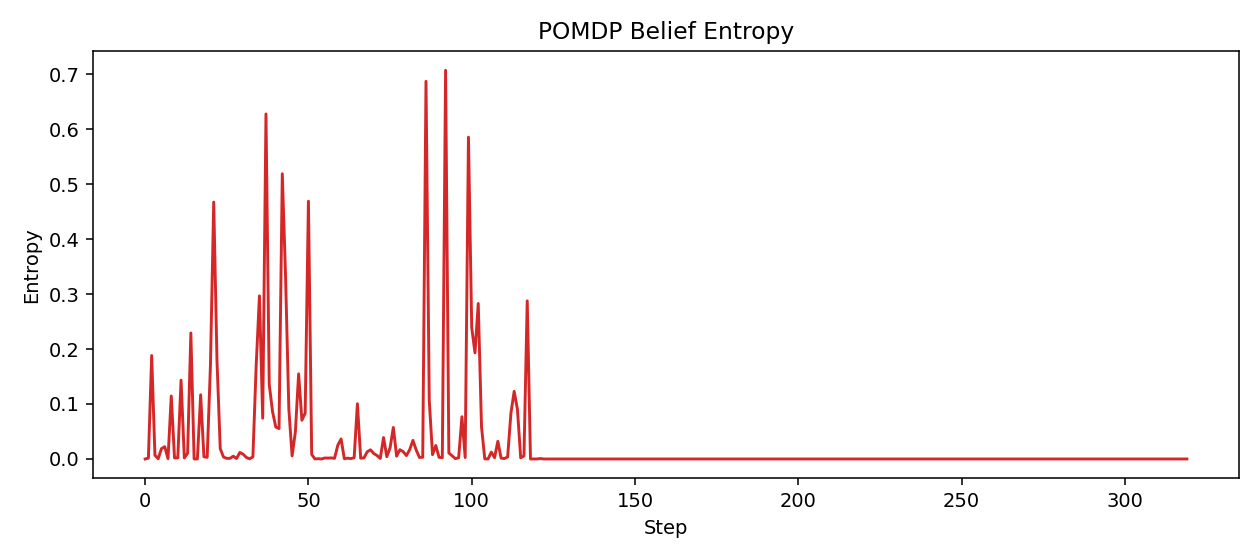
\includegraphics[width=0.9\textwidth]{results/sections/pomdp/pomdp_belief_entropy.png}
    \caption{Entropie de croyance $H(b_t)$ au fil du temps. Les pics correspondent
    aux instants de transition entre états latents.}
    \label{fig:belief_entropy}
\end{figure}

\subsection{Extension non-Markovienne : multiplicateur de risque}

Pour capturer l'effet de l'historique (dégradation cumulée non reflétée dans l'état courant),
on définit une feature mémoire~:
\[
\rho_t = \left(1 + \min\!\left(0{,}5,\,\frac{\text{âge}}{1000}\right)\right)
         \cdot \left(1 + \min\!\left(0{,}7,\,\frac{\text{ECC\_cumulé}}{50}\right)\right).
\]
Ce multiplicateur amplifie la probabilité de transition vers $FP$ dans la ligne courante de $\mathbb{P}$.

\begin{figure}[H]
    \centering
    
\includegraphics[width=0.9\textwidth]{results/mandatory_plots/non_markov_risk_multiplier.png}
    \caption{Multiplicateur de risque non-Markovien (âge + cumul ECC).
    Dépasse $2\times$ en fin de trace sans maintenance.}
    \label{fig:non_markov_multiplier}
\end{figure}

% ============================================================
\section{Protocole Expérimental et Résultats Consolidés}
% ============================================================

\subsection{Reproductibilité}

Le code est entièrement reproductible~:
\begin{itemize}
  \item \texttt{python -m src.main --mode full} : exécution complète (graine 7).
  \item \texttt{python -m src.run\_section --section all} : génère tous les fichiers de section.
  \item \texttt{python -m src.generate\_assets --runs 30} : génère le bundle multi-runs.
\end{itemize}
L'environnement est spécifié dans \texttt{requirements.txt}.
Les graines aléatoires sont fixées (\texttt{seed=7} pour la trace de référence,
graines 101--130 pour les 30 runs multi-runs).

\subsection{Résultats consolidés}

\begin{center}
\begin{tabular}{lc}
\toprule
Métrique & Valeur \\
\midrule
MTTF DTMC depuis Healthy (pas) & 78,93 \\
Retour moyen Q-learning (300 épisodes) & 63,87 \\
Retour moyen SARSA (300 épisodes) & 67,21 \\
Gain moyen R-learning ($\rho$) & 0,667 \\
$V_{TD(0)}(\text{Healthy})$ & 14,02 \\
$V_{TD(\lambda)}(\text{Healthy})$ & 13,82 \\
Exactitude Viterbi & 99,69\,\% \\
Entropie Forward moyenne & 0,0285 nats \\
Entropie POMDP max & 0,71 nats \\
Accord POMDP/MDP & 97,3\,\% \\
\bottomrule
\end{tabular}
\captionof{table}{Récapitulatif des métriques clés. Source~: \texttt{results/summary.csv}
et fichiers de sections.}
\end{center}

\subsection{Analyse de sensibilité}

Une analyse de sensibilité sur $\gamma \in \{0{,}85, 0{,}90, 0{,}95, 0{,}98\}$
et un facteur d'échelle de défaillance $\in \{0{,}8, 1{,}0, 1{,}2, 1{,}5\}$
est sauvegardée dans \texttt{results/sensitivity.csv}.
Elle montre que le score de politique est robuste pour $\gamma \geq 0{,}90$
mais se dégrade significativement pour des taux de défaillance $1{,}5\times$.

% ============================================================
\section{Conclusion et Perspectives}
% ============================================================

Ce rapport présente une modélisation stochastique complète de la disponibilité d'un cluster
GPU H100 pour l'entraînement de LLM, calibrée sur des données réelles vérifiables.
Les sources (\href{https://arxiv.org/pdf/2407.21783}{arXiv:2407.21783}
et \href{https://arxiv.org/pdf/2503.11901}{arXiv:2503.11901}) fournissent les statistiques
de défaillance directement utilisées pour dériver les matrices DTMC, CTMC,
et les paramètres d'émission HMM.

Tous les algorithmes requis sont implémentés et validés~:
Forward, Backward, Viterbi, Baum-Welch (EM), value iteration (MDP),
Q-learning, SARSA, R-learning, TD(0), TD($\lambda$), et mise à jour de croyance (POMDP).

\subsection{Limites}

\begin{itemize}
  \item Les probabilités de transition sont calibrées sur des statistiques agrégées au niveau cluster~;
        une estimation individuelle par GPU nécessiterait des traces DCGM privées.
  \item La résolution POMDP est approximative (point-based)~;
        PBVI ou SARSOP donneraient des garanties formelles d'optimalité.
  \item L'hypothèse de Markov au niveau cluster ignore les corrélations inter-GPU
        (pannes en cascade via NVLink).
  \item La stationnarité de $\mathbb{P}$ dans le temps est une approximation~;
        la dégradation progressive des GPU brise cette hypothèse sur le long terme.
\end{itemize}

\subsection{Perspectives}

\begin{itemize}
  \item Calibration sur télémétrie réelle via NVIDIA DCGM + logs XID (disponibles sur clusters internes).
  \item Modèles POMDP profonds (Deep POMDP) pour observations continues haute-dimension.
  \item Validation sur scénarios multi-nœuds avec corrélations NVLink.
  \item Apprentissage en ligne des paramètres HMM par Baum-Welch adaptatif.
  \item Extension à la planification de maintenance préventive (CBM) avec contraintes de coût.
\end{itemize}

\FloatBarrier
\clearpage

% ============================================================
\section{Références}
% ============================================================

\begin{enumerate}
  \item Grattafiori, A. et al.\ (2024).
        \textit{The Llama 3 Herd of Models}.
        arXiv:2407.21783.
        \href{https://arxiv.org/pdf/2407.21783}{\texttt{https://arxiv.org/pdf/2407.21783}}\\
        \textbf{Usage~:} Source principale. Table~5 (p.\,7)~: 419 pannes sur 54 jours,
        16\,384 GPU H100. Décomposition par type de défaillance utilisée directement
        pour calibrer $\mathbb{P}$ et $\mathbb{A}$.

  \item Cui, S. et al.\ (2025).
        \textit{Story of Two GPUs: Characterizing the Resilience of Hopper H100 and Ampere A100 GPUs}.
        arXiv:2503.11901. SC'25.
        \href{https://arxiv.org/pdf/2503.11901}{\texttt{https://arxiv.org/pdf/2503.11901}}\\
        \textbf{Usage~:} Source secondaire. Table~1~: MTBE H100 = 1,9\,h système,
        292\,h/nœud. Disponibilité 99,5\,\%. 11,7M heures GPU sur Delta (NCSA/UIUC).
        Figure~1~: XID\,48 et XID\,31 comme erreurs dominantes.

  \item El Afia, A.\ (2026).
        \textit{Apprentissage Probabiliste~: Chaînes de Markov, HMM, MDP, RL}.
        Supports de cours, Master Science de Données, ENS Martil.

  \item Epoch AI.\ (2024).
        \textit{Hardware Failures Won't Limit AI Scaling}.
        \href{https://epoch.ai/blog/hardware-failures-wont-limit-ai-scaling}{\texttt{epoch.ai/blog/...}}\\
        MTTF par GPU H100 $\approx$ 50\,000\,h~; validation de la formule cluster MTTF = 3\,h
        à 16\,384 GPU.

  \item NVIDIA.\ (2024).
        \textit{XID Errors --- NVIDIA Documentation}.
        \href{https://docs.nvidia.com/deploy/pdf/XID_Errors.pdf}{\texttt{docs.nvidia.com/deploy/pdf/XID\_Errors.pdf}}\\
        Définition et classification des codes XID utilisés dans la matrice d'émission.

  \item NVIDIA.\ (2024).
        \textit{NVIDIA Data Center GPU Manager (DCGM)}.
        \href{https://developer.nvidia.com/dcgm}{\texttt{developer.nvidia.com/dcgm}}\\
        Interface de télémétrie GPU~: source des signaux ECC, température, utilisation.

  \item Xiong, Y. et al.\ (2024).
        \textit{SuperBench: Improving Cloud AI Infrastructure Reliability with Proactive Validation}.
        USENIX ATC'24.
        \href{https://www.usenix.org/system/files/atc24-xiong.pdf}{\texttt{usenix.org/...}}

  \item Barto, A.G., Sutton, R.S.\ (2018).
        \textit{Reinforcement Learning: An Introduction} (2nd ed.).
        MIT Press.

  \item Rabiner, L.R.\ (1989).
        A Tutorial on Hidden Markov Models and Selected Applications in Speech Recognition.
        \textit{Proceedings of the IEEE}, 77(2), 257--286.

  \item Kaelbling, L.P., Littman, M.L., Cassandra, A.R.\ (1998).
        Planning and Acting in Partially Observable Stochastic Domains.
        \textit{Artificial Intelligence}, 101(1--2), 99--134.

  \item Das, R. et al.\ (2025).
        \textit{Characterizing GPU Resilience and Impact on AI/HPC Systems}.
        arXiv:2503.11901v1.
        \href{https://arxiv.org/html/2503.11901v1}{\texttt{arxiv.org/html/2503.11901v1}}

  \item Revisiting Reliability in Large-Scale Machine Learning Research Clusters.
        arXiv:2410.21680.
        \href{https://arxiv.org/pdf/2410.21680}{\texttt{arxiv.org/pdf/2410.21680}}

  \item CoreWeave.\ (2025).
        \textit{Training Benchmarks Whitepaper}.
        \href{https://cdn.prod.website-files.com/62bc66d283fd9c34ffec780a/689fa33a0e99f19c11c8ecbe_CoreWeave\%20Training\%20Benchmarks\%20Whitepaper\%20August\%202025.pdf}{\texttt{coreweave.com/...}}

  \item Performance Analysis for a Degrading System with Markov Model.
        ResearchGate.
        \href{https://www.researchgate.net/publication/363336255}{\texttt{researchgate.net/...}}
\end{enumerate}

\end{document}